\chapter{Behavior Mapping}

\section{Computing Behavioral Embeddings}
\citet{mcinnes_umap_2020} \citet{mcinnes_hdbscan_2017} \citet{campello_density-based_2013}

\subsection{Supervised Disparate Embeddings}
\begin{figure}[ht]
	\centering
	\begin{subfigure}[b]{0.325\linewidth}
		\centering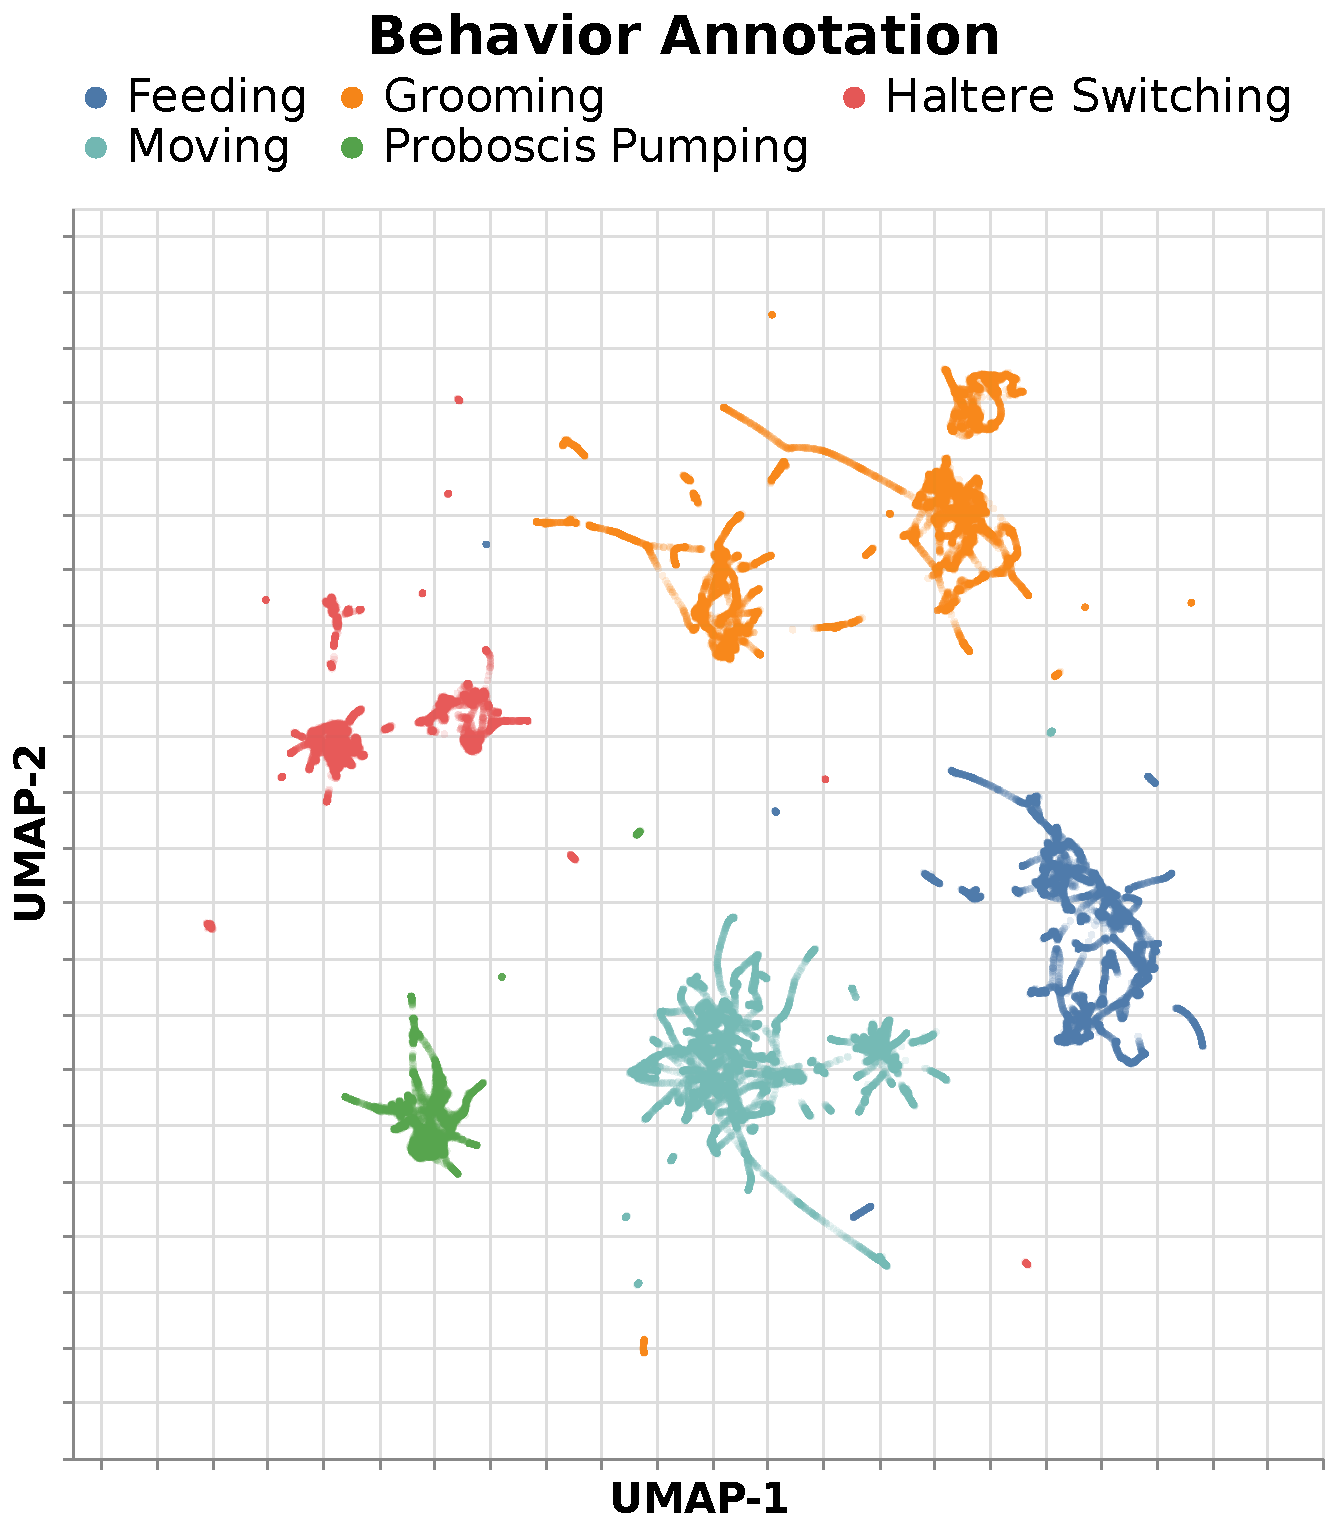
\includegraphics[width=\linewidth]{figures/scatter2D-FlyF15-08182021173222-supervised_disparate-DA-wAnn.pdf}
		\caption{\label{figure:supervised-disparate-DAnn-wAnn}}
	\end{subfigure}%
	\hfill
	\begin{subfigure}[b]{0.325\linewidth}
		\centering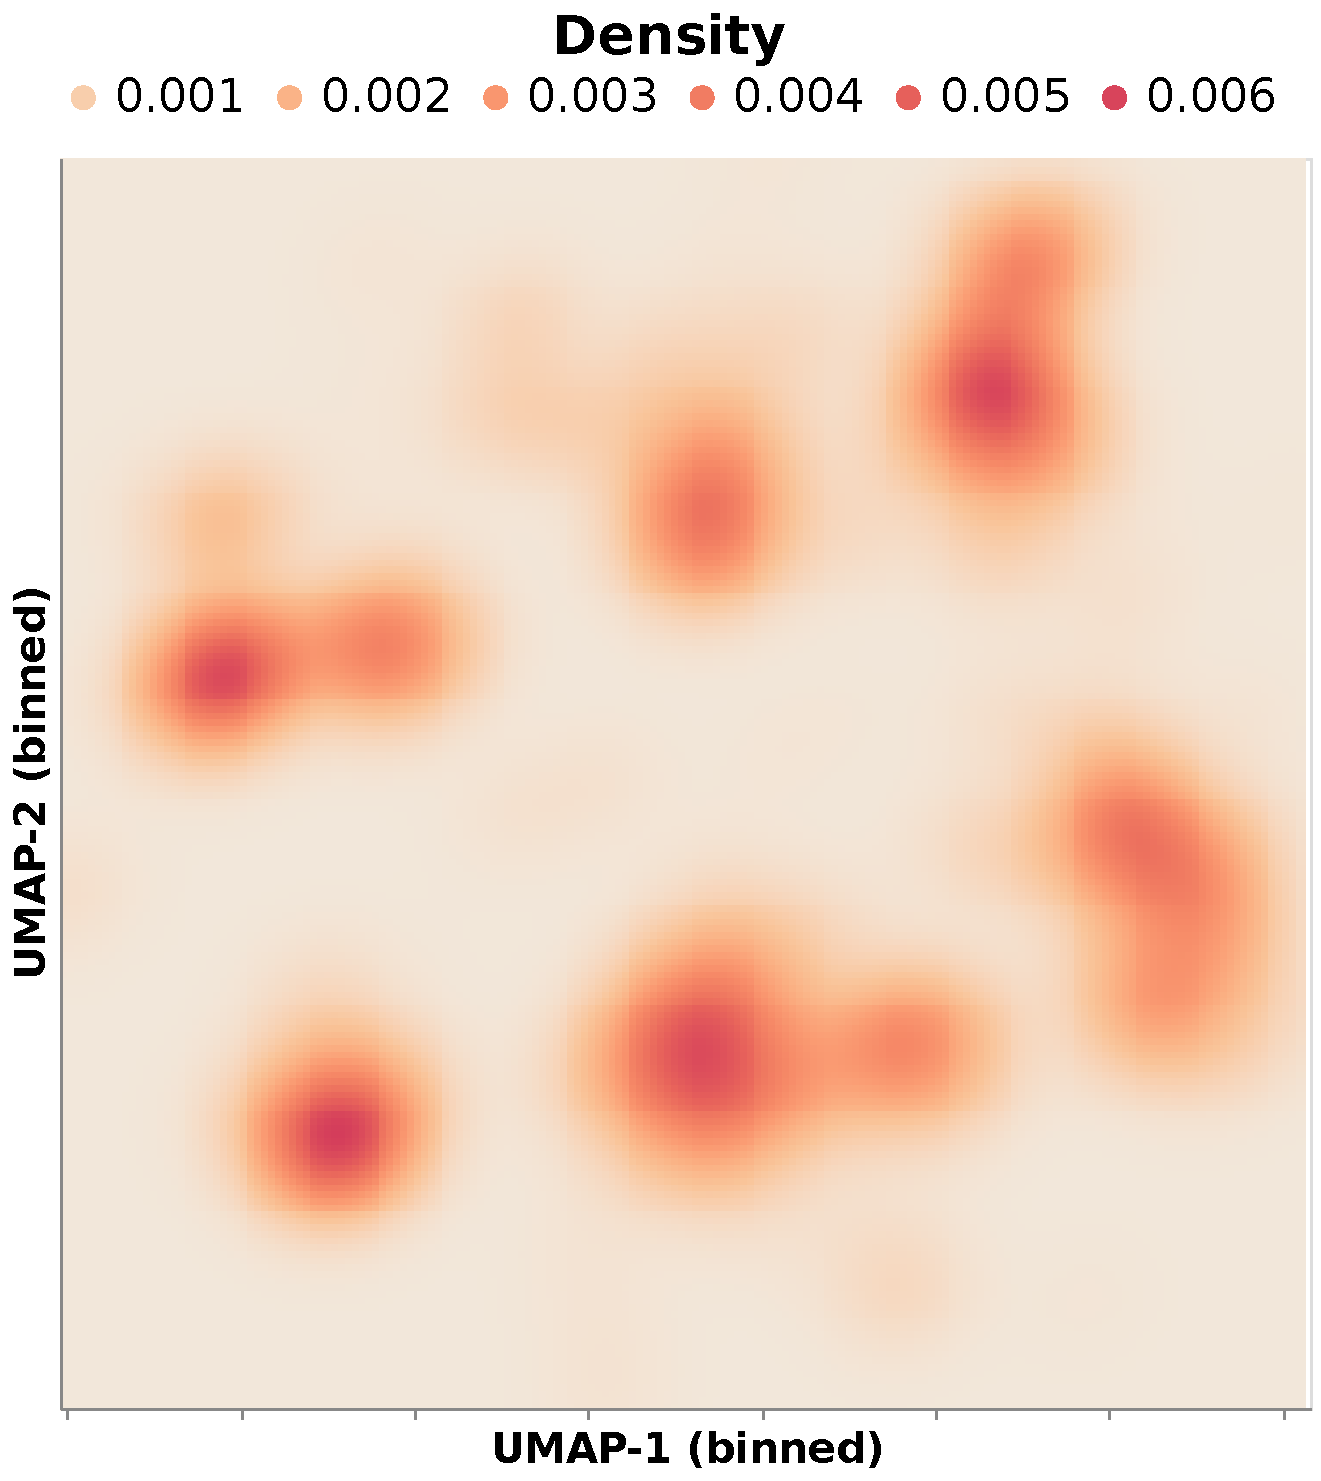
\includegraphics[width=\linewidth]{figures/densmap2D-FlyF15-08182021173222-supervised_disparate-DA-denstiy.pdf}
		\caption{\label{figure:supervised-disparate-DAnn-density}}
	\end{subfigure}%
	\hfill
	\begin{subfigure}[b]{0.325\linewidth}
		\centering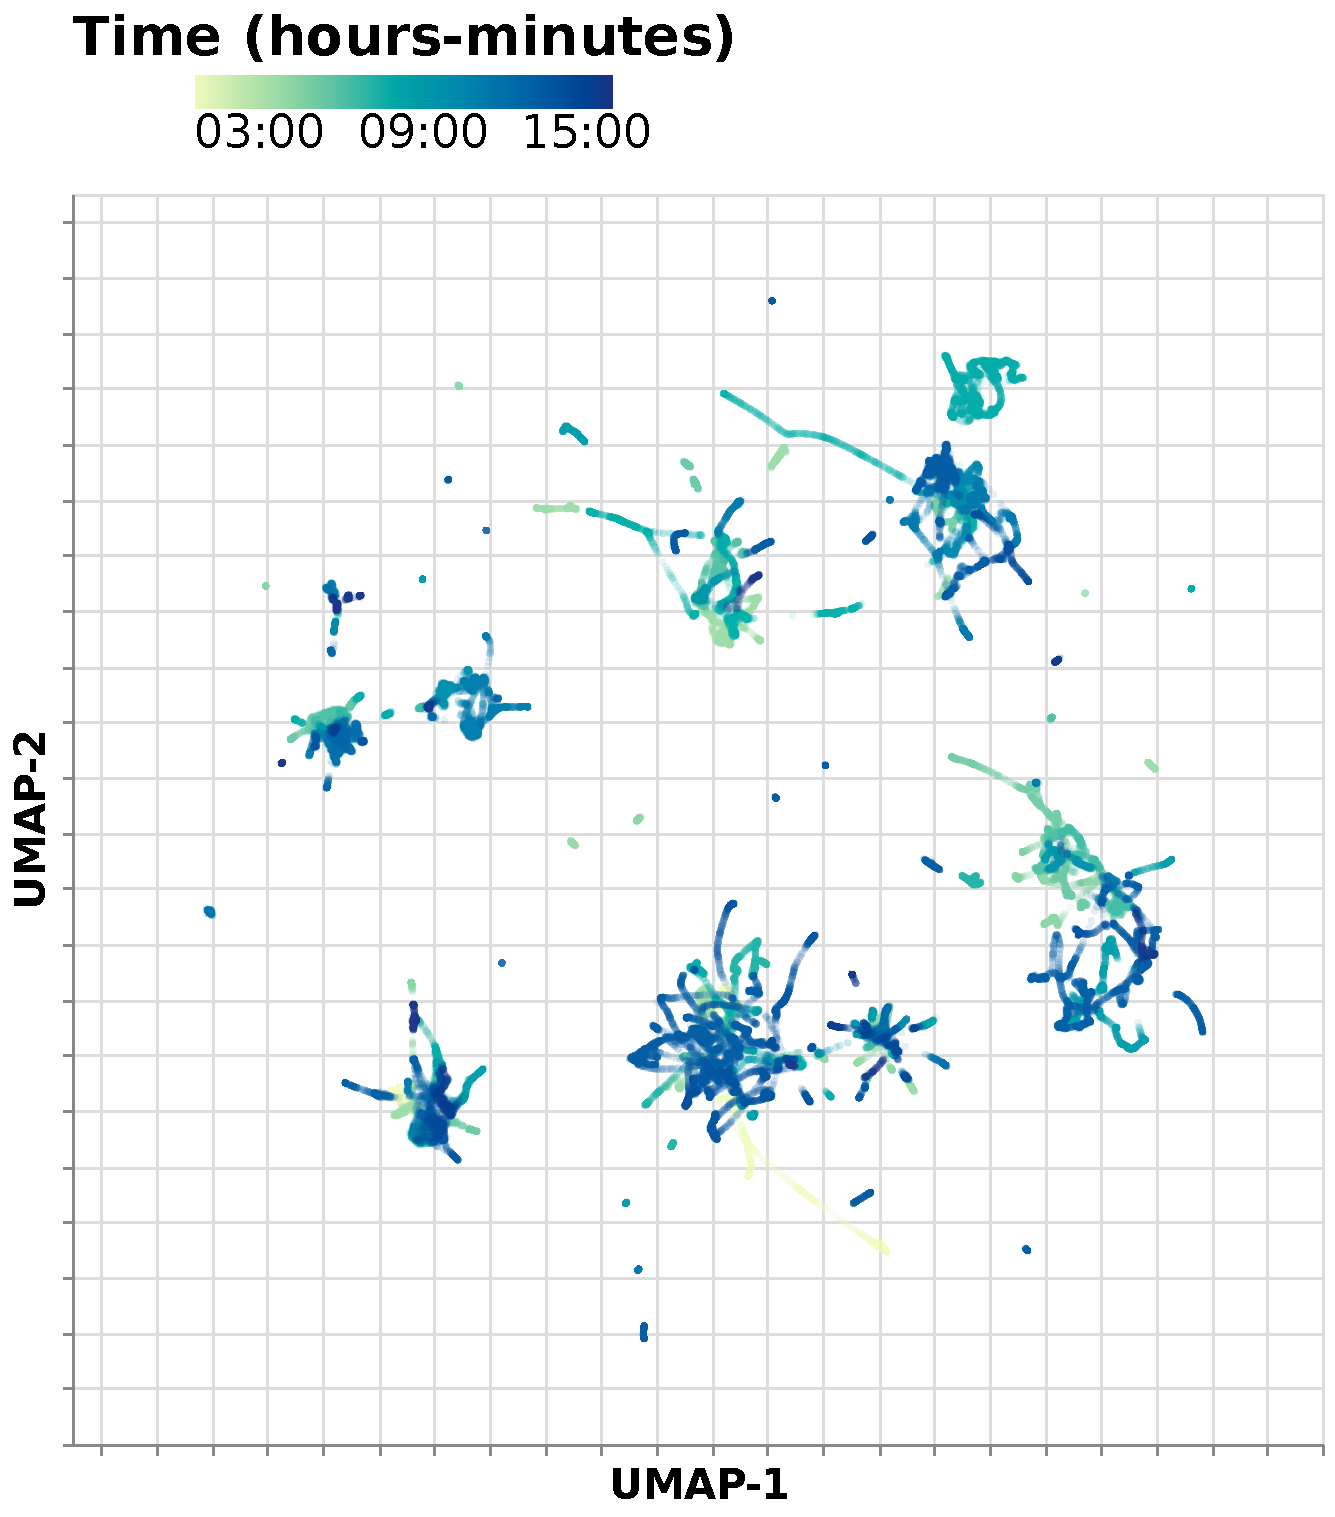
\includegraphics[width=\linewidth]{figures/scatter2D-FlyF15-08182021173222-supervised_disparate-DA-wTemporal.pdf}
		\caption{\label{figure:supervised-disparate-DAnn-wTemporal}}
	\end{subfigure}
	\caption{Supervised Disparate Embedding.}
\end{figure}

\NOTE{
	We compute Supervised-UMAP embeddings separately for each experiment.
	Computing supervised embeddings is only possible for annotated experiments.
	This is useful for exploring behavioral sub-categories.
	For instance, one annotation category, e.g. "grooming", can be consisted of two different clusters in the behavioral embedding space.
	We can further investigate how high-level behavioral annotations contain different but similar behaviors.
}

\subsection{Supervised Joint Embeddings}
\NOTE{
	We compute Supervised-UMAP embeddings of all annotated experiments together.
	There is no specific benefit or use case (except visualization purposes) for computing this.
	The resulting embedding usually is not homogeneous in terms of fly experiments.
	Different flies do not mix well in the behavioral space.
}

\subsection{Unsupervised Disparate Embeddings}
\NOTE{
	For each experiment, we compute a usual unsupervised embedding separately.
}

\subsection{Unsupervised Joint Embedding}
\NOTE{
	We compute a single behavioral embedding using all experiments.
	The problem with this approach is that embedding space is too crowded and thus we can not find meaningful and homogeneous clusters right away.
	This embedding might be useful for visualization purposes.
}

\subsection{Semi-supervised Pair Embeddings}
\NOTE{
	This is the novel and most useful embedding approach that we finally utilize to label unannotated experiments using annotated ones.
	We compute an embedding for each annotated and unannotated pair.
	For example, if there are $N_A$ annotated experiments and $N_U$ unannotated experiments we compute $N_A \cdot N_U$ embeddings in total.
	There are number of advantageous of this approach.
	Especially when, an behavioral repertoire of an annotated an unannotated are similar, resulting embedding is easy to interpret and use for clustering etc.
}
\section{Soft Clustering of Behavioral Embeddings}
\NOTE{
	We always use soft clustering feature of HDBSCAN, since it is very beneficial to have a composite assignment for a data-point.
	For example, 0.7 grooming, 0.3 proboscis pumping may indicate that those two behaviors are simultaneously exhibited or a combination of both is exhibited etc.
	We can always take $\argmax$ if a categorical label is needed.
}

\subsection{Disparate Clustering}

\NOTE{
	If embedding is a disparate embedding, then we directly cluster each of them separately.
	If a joint embedding or pair embedding will be clustered, then experiments need to be extracted from the embedding space first and then they need to be clustered separately.
}

\subsection{Joint Clustering}
\NOTE{
	This is only applicable to joint and pair embeddings. We cluster all experiments in the behavioral embedding together.
}

\subsection{Crosswise Clustering}
\NOTE{
	This is again only applicable to joint and pair embeddings.
	For joint embeddings, we exclude a sub-group of experiments.
	For pair embeddings, we exclude one of the pair experiments.
	Then rest of the embedding is clustered and clusters are formed.
	Finally for each excluded embedding, soft cluster memberships vectors are computed based on the formed clusters.
}

\section{Computing Behavioral Correspondences}

\subsection{Mapping Clusters to Behavioral Categories}

\NOTE{
	If a clustering contains annotated experiments, we map that clusters in that clustering to a behavioral composition as follows ({\it subject to change, there are couple of alternatives})
	\begin{equation}
		m_\alpha = \frac{\textnormal{number of frames with annotation }\alpha \textnormal{ in the cluster}}{\textnormal{total number of frames with annotation }\alpha}.
	\end{equation}
	So for each cluster, we end up with a vector $\mathbf{m}=(m_\alpha)$, represent it behavioral composition.
}

\subsection{Computing Behavioral Scores}
\NOTE{
	Behavioral score of unannotated experiment will be computed using clustering membership score and behavioral composition mapping of those clusters.
	For example, using semi-supervised pair embeddings and crosswise clustering; one can compute behavioral scores for a frame as follows;
	\begin{equation}
		y_\alpha = \sum_{c=0}^C m^c_\alpha
	\end{equation}
	where $C$ is the number of clusters, $\mathbf{m}^c$ is the behavioral composition of cluster $c$.
	As a result, for each frame we end up with a behavioral score vector $\mathbf{y}=(y_\alpha)$.
}
